\section*{¿Qué es Indusmoney?}
IndusMoney opera como la Empresa 6 dentro del Grupo 7, y su estrategia inicial se ha centrado en el crecimiento paulatino de su capacidad operativa y su presencia comercial en mercados clave.  

La compañía se enfoca en tres segmentos de mercado principales: el tradicional mercado europeo (UE), que sirve como base principal; el mercado Nafta, que se está consolidando como una vía de expansión geográfica; y el canal de Internet, considerado el pilar de crecimiento futuro.  

IndusMoney comercializa actualmente tres líneas de productos: Producto 1, Producto 2 y Producto 3, sobre los cuales se han realizado inversiones de Investigación y Desarrollo (I+D) en todos los trimestres analizados. 

\section*{Análisis de histórico}
Antes de formular su estrategia actual en el GMC, IndusMoney realizó un análisis exhaustivo de sus resultados históricos. Este estudio previo permitió identificar los puntos fuertes y las áreas de mejora (como la fluctuación de la rentabilidad). El análisis se centró en conocer las dinámicas de precios, la evolución de la demanda por mercado y producto, la gestión de inventarios, y, fundamentalmente, la estructura de ingresos y costes reflejada en los estados. 

\section*{Ingresos por Ventas y Rentabilidad}
El volumen de negocio experimentó un crecimiento espectacular desde el inicio (0€ en Trm 2.0/2016) hasta alcanzar su máximo de 1.329.434€ en Trm 2.0/2017. Sin embargo, el esfuerzo de lanzamiento y la inversión en estructura generaron grandes pérdidas operativas iniciales, con el Beneficio Neto cayendo a un mínimo de -16.919€ en Trm 3.0/2016. La rentabilidad mostró signos de estabilidad en el Trm 4.0/2016 con un beneficio de 72.426€, para finalmente consolidar su mejor resultado con un Beneficio Neto de 121.419€ en el último trimestre. 

\begin{figure}[h]
  \centering
  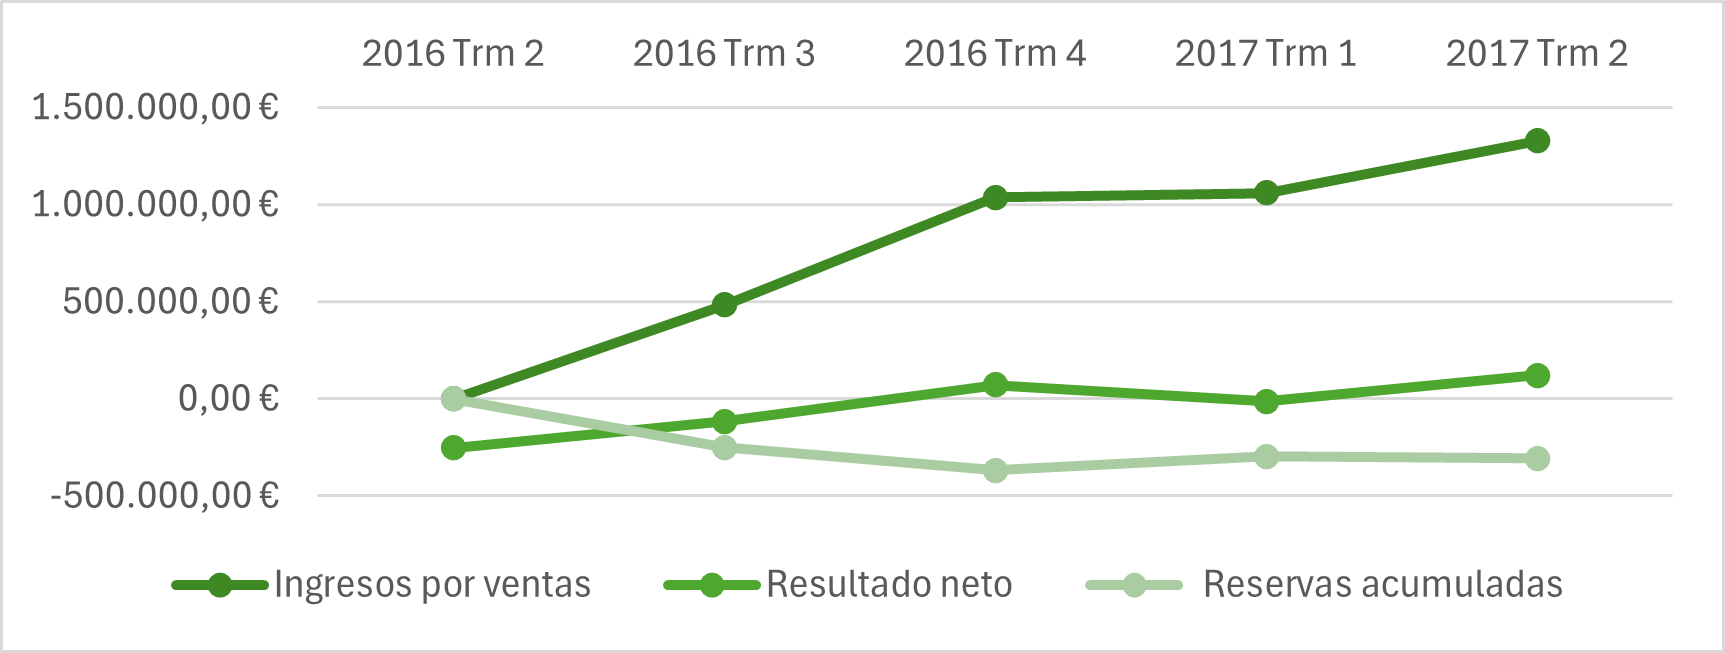
\includegraphics[width= \columnwidth]{Imagenes/introduccion_ingresosbeneficioreservas.png}
\end{figure}

\section*{Patrimonio y Liquidez}
La mejora en la rentabilidad es crítica, ya que ha permitido a la empresa revertir la tendencia negativa de sus Reservas Acumuladas, pasando de un mínimo de -307.504€ en Trm 1.0/2017 a -186.085€ en el Trm 2.0/2017, mejorando significativamente el Patrimonio Neto. La liquidez se ha mantenido muy sólida en todo el periodo, con el Efectivo e Inversiones superando los 1.8 millones de euros al cierre del Trm 2.0/2017, asegurando la capacidad de inversión futura. 

\section*{Análisis de precios}
\subsection*{Producto 1: Liderazgo en el Ajuste de Precios}
Muestra el crecimiento de precios más agresivo, pasando de 285€ a 325€ (+14\%) en los últimos dos trimestres. Este aumento está directamente relacionado con la aplicación de una Mejora Mayor, permitiendo a la empresa capitalizar el valor añadido del producto para impulsar la rentabilidad. 

\begin{figure}[h]
  \centering
  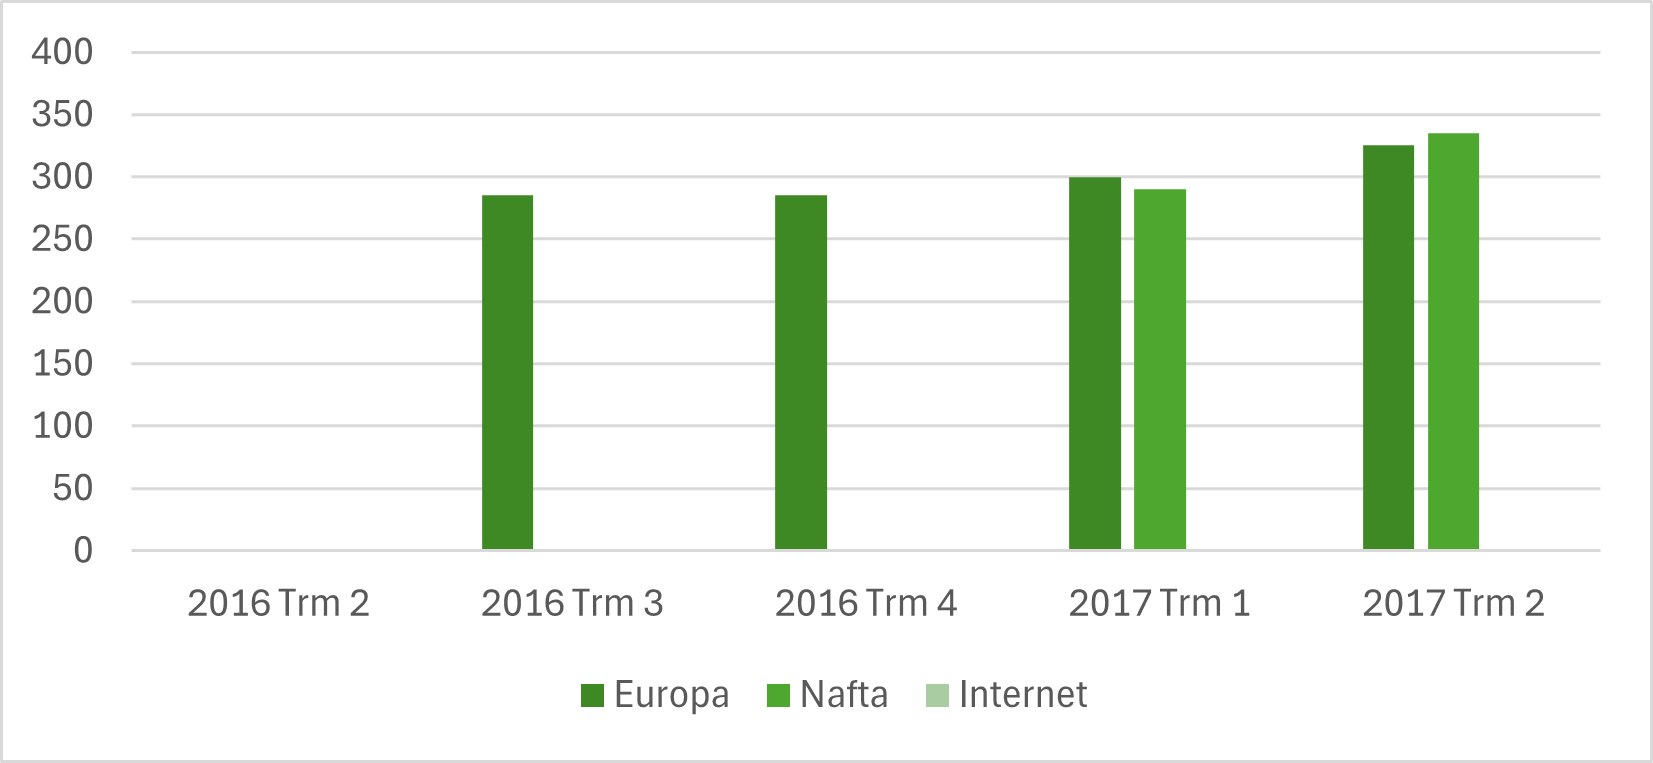
\includegraphics[width= \columnwidth]{Imagenes/introduccion_producto1.png}
\end{figure}

\subsection*{Producto 2: Mantenimiento y Recuperación de Valor}
Mantuvo la estabilidad en 450€ durante el inicio de la operación, buscando volumen de ventas. El ajuste se realizó tardíamente en el Trm 2.0/2017, con un aumento significativo a 490€ (+9\%), reflejando una decisión de recuperar valor y margen una vez asegurada la posición en el mercado.

\begin{figure}[h]
  \centering
  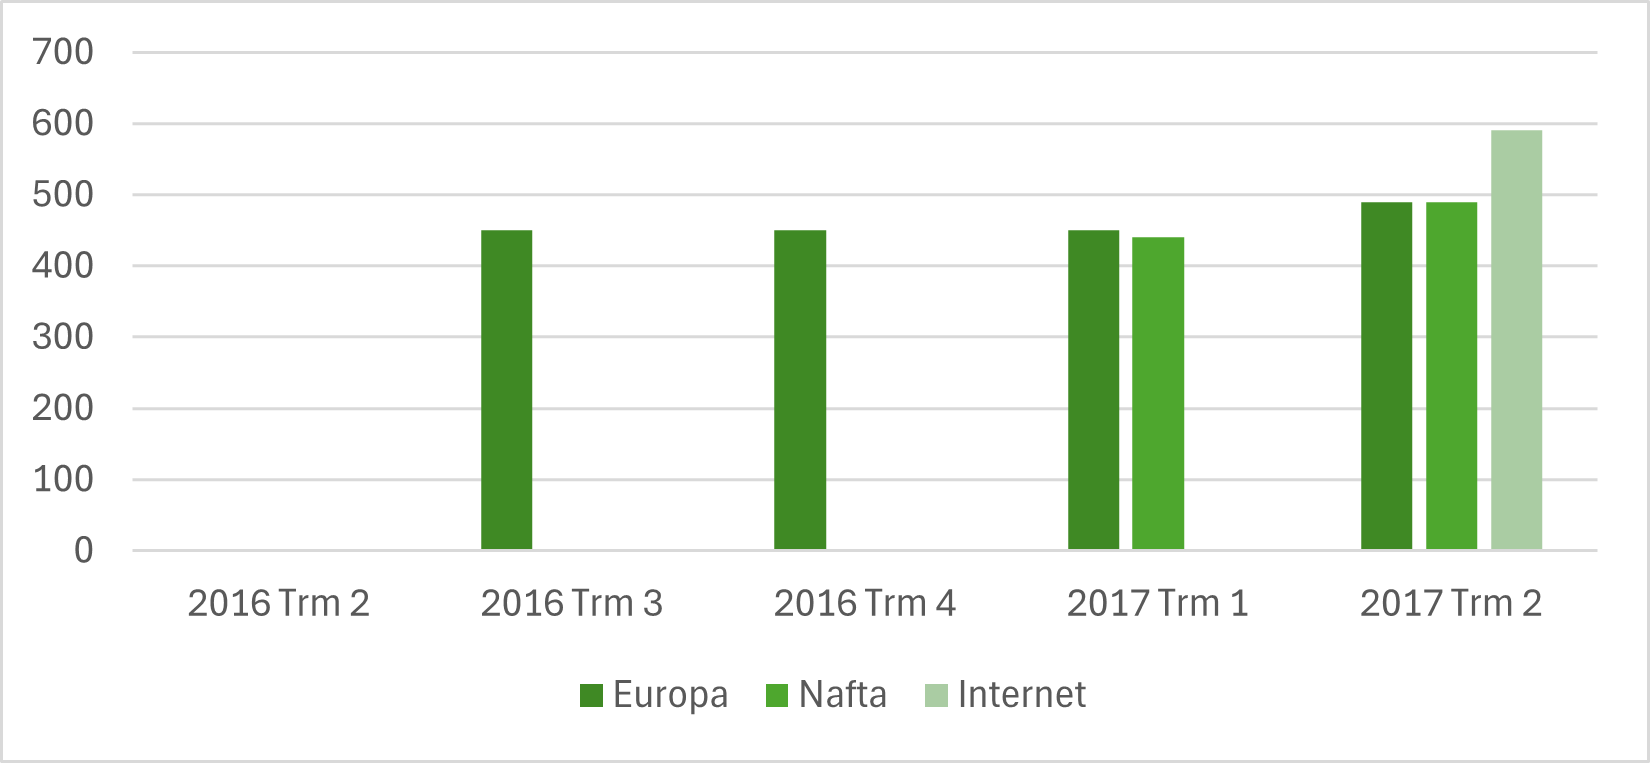
\includegraphics[width= \columnwidth]{Imagenes/introduccion_producto2.png}
\end{figure}

\subsection*{Producto 3: Ajustes Moderados y Estabilidad}
Presenta la evolución más cautelosa, con ajustes muy moderados de 680€ a 700€. Esta estrategia indica que la empresa ha priorizado mantener la demanda y la competitividad en este segmento de mayor coste, limitando la sensibilidad del mercado a los cambios de precio. 

\begin{figure}[h]
  \centering
  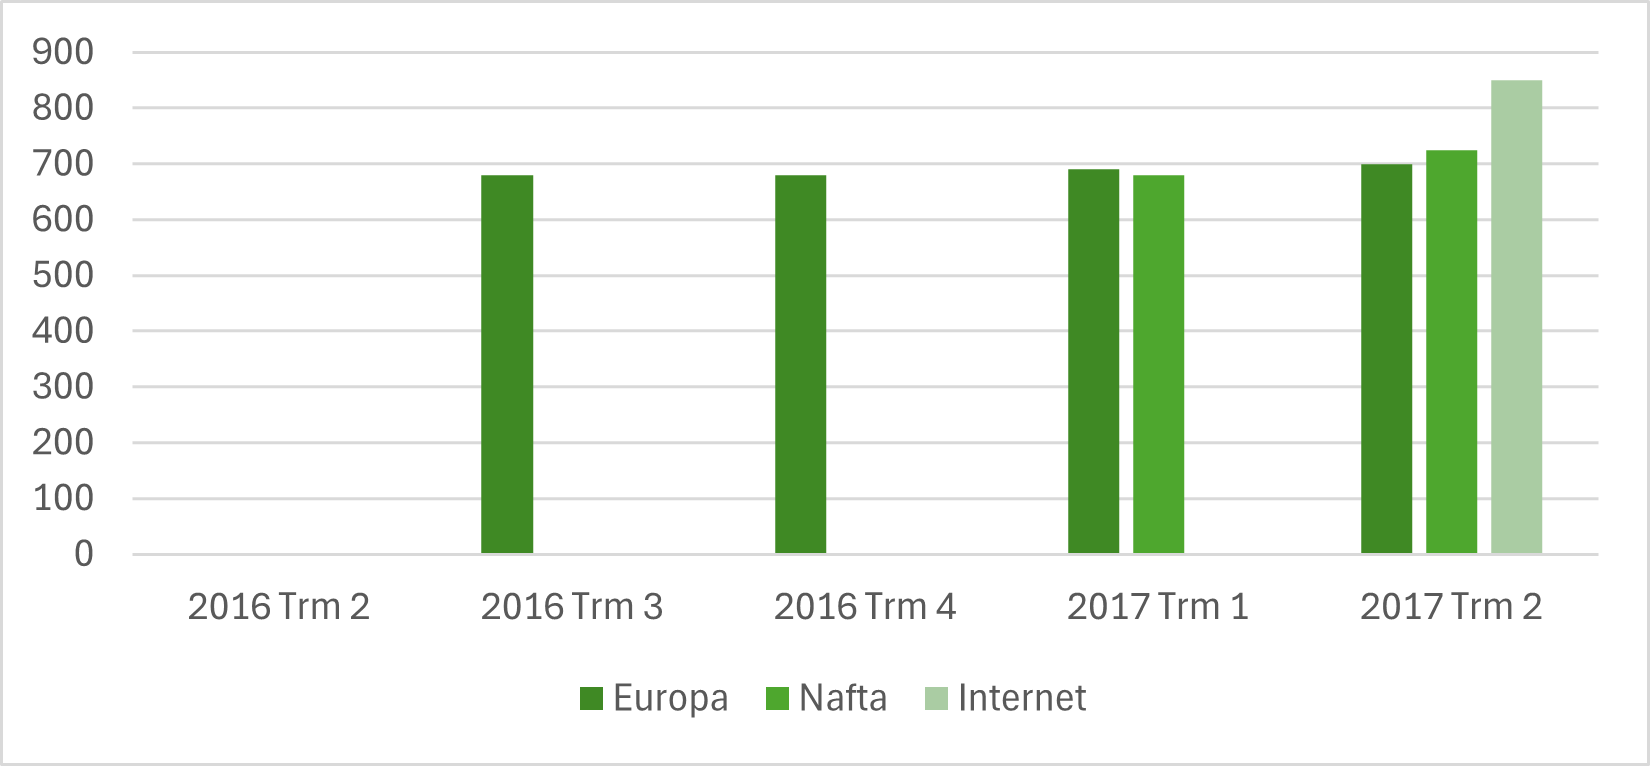
\includegraphics[width= \columnwidth]{Imagenes/introduccion_producto3.png}
\end{figure}
